%
% google.tex -- Einstiegsproblem zur Behandlung von Google-Matrizen
%
% (c) 2020 Prof Dr Andreas Müller, Hochschule Rapperswil
%
\section{Google-Matrix
\label{buch:section:google-matrix}}
\rhead{Google-Matrix}
Das Internet besteht aus einer grossen Zahl von Websites, etwa 400~Millionen
aktiven Websites, jede besteht aus vielen einzelnen Seiten.
\index{Internet}%
Es ist daher angemessen von $N\approx 10^9$ verschiedenen Seiten auszugehen.
Eine natürliche Sprache umfasst dagegen nur einige 100000 bis Millionen
von Wörtern.
Ein durchschnittlicher Sprecher englischer Muttersprache verwendet nur etwa
50000 Wörter.
Die Zahl der Wörter, die auf den $N$ Seiten vorkommen können, ist also
viel kleiner als die Zahl der zur Verfügung stehenden Wörter.
Ein einzelnes Wort wird daher notwendigerweise auf einer grossen Zahl
von Seiten vorkommen.
Eine Suche nach einem bestimmten Wort wird in der überwiegenden Zahl
der Fälle derart viele Treffer zurückgeben, dass das Suchresultat
nur dann nützlich sein kann, wenn eine zusätzliche Informationsquelle
ermöglicht, die Treffer in eine sinnvolle Ordnung zu bringen.

Genau dieses Problem stellte sich den vielen traditionellen Suchmaschienen
in der ersten grossen Boomphase des Internets.
Traditionelle Information-Retrieval-Systeme operieren auf einem relativ
\index{Information-Retrieval}%
kleinen Dokumentbestand und gehen davon aus, dass bereits wenige, spezifische
Wörter nur in einem kleinen Teil des Dokumentbestandes vorkommen und damit
eine übersichtliche Treffermenge ergeben.
Die Einengung der Treffermenge dank der Suche nach einzelnen Wörtern
bedeutet aber auch, dass nach Synonymen oder alternative Formen eines
Wortes separat gesucht werden muss, was die Übersichtlichkeit wieder
zerstört.
\index{Treffermenge}%

%
% Ein Modell für Webseitenbesucher
%
\subsection{Ein Modell für Webseitenbesucher
\label{buch:subsection:modell-fuer-webseitenbesucher}}
\begin{figure}
\centering
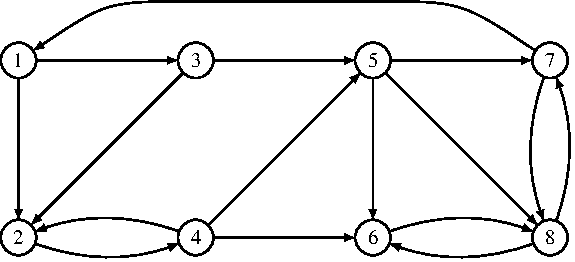
\includegraphics{chapters/80-wahrscheinlichkeit/images/internet.pdf}
\caption{Modell-Internet als Beispiel für die Link-Matrix und die Google-Matrix.
\label{buch:figure:modellinternet}}
\end{figure}

Selbst das kombinierte Vorkommen von Wörtern oder Begriffen alleine reicht
nicht aus, um die Seiten zum Beispiel einem Fachgebiet zuzuordnen.
Dazu muss eine externe Informationsquelle angezapft werden.
Bei traditionellen Dokumenten liefert der Kontext, in dem ein
Dokument erfasst wurde, solche ergänzenden Informationen.
Eine Publikation in einem Fachjournal ordnet einen Text einem Fachgebiet zu.
Im World-Wide-Web liefert die Link-Struktur diesen Kontext.
\index{Link}%
Dokumente zu ähnlichen oder verwandten Themen werden bevorzugt
untereinander verlinkt sein.

Gesucht ist jetzt also ein Modell, welches objektiv die Linkstruktur
bewertet und daraus eine Rangordnung der Suchresultate ableitet.
Die Linkstruktur kann natürlich als gerichteter Graph betrachtet und 
mit Hilfe der Adjazenzmatrix~\eqref{buch:graphen:eqn:adjazenzmatrixgerichtet}
\index{Adjazenzmatrix}%
eines gerichteten Graphen beschrieben werden.
Dies trägt jedoch der Anzahl der Wahlmöglichkeiten nicht Rechnung.
Eine Website mit nur einem Link auf die Seite $j$ gibt der Seite $j$
mehr Gewicht als eine Seite mit vielen Links, unter denen der Link
auf die Seite $j$ einer von Vielen ist.
Im Beispiel-Internet der Abbildung~\ref{buch:figure:modellinternet}
signalisiert die Seite $6$ mit nur einem Link auf die Seite $8$
viel deutlicher, dass $8$ eine wichtige Seite ist, also die die
Seite $5$ tut, die auch noch zwei andere Links enthält.
Wir können diesen Unterschied berücksichtigen, indem wir zu einem
Wahrscheinlichkeitsmodell übergehen, was wir im folgenden Abschnitt
tun werden.

%
% Wahrscheinlichkeitsinterpretation
%
\subsection{Wahrscheinlichkeitsinterpretation
\label{buch:subsection:wahrscheinlichkeitsinterpretation}}
Ein Internetbesucher kann eine grosse Zahl von Seiten besuchen.
In diesem Abschnitt soll ein Modell entwickelt werden, welches die
Wahrscheinlichkeit zu ermitteln gestattet, dass der Besucher auf
einer bestimmten Seite landet.

\subsubsection{Ereignisse und Wahrscheinlichkeiten}
Wir bezeichnen mit $S_i$ das Ereignis, dass sich der Besucher auf
der Seite mit der Nummer $i$ befindet, wobei $i=1,\dots,N$.
Gesucht ist die Wahrscheinlichkeit $P(S_i)$.
Ohne weitere Information müssten wir davon ausgehen, dass jede Seite
etwa gleich wahrscheinlich ist, dass also $P(S_i) = 1/N$.

Wir wissen jedoch mehr.
Wir wissen, dass der Besucher die verschiedenen Seiten zu einem guten 
Teil dadurch findet, dass er Links folgt.
Die Wahrscheinlichkeit $P(S_i)$ verändert sich also, wenn die Zahl der
Links ansteigt, die auf die Seite $i$ verweisen.
Zur Beschreibung dieses Phänomens brauchen wir die zusätzliche Ereignisse
$S_i'$, die mit Wahrscheinlichkeit $P(S'_i)$ eintreten, wenn sich der
Besucher nach Navigation entlang eines Links auf der Seite $i$ befindet.

Wir nehmen jetzt zusätzlich an, dass eine grosse Zahl von Besuchern über
lange Zeit ungefähr nach den gleichen Dingen suchen und sich daher
auf die gleiche Weise auf den verschiedenen Seiten verteilen und dass
insbesondere die Verteilung stationär ist, dass also $P(S_i) = P(S'_i)$
gilt.
\index{Suchmaschine}%
Suchmaschinen wie Google gehen davon aus, dass alle Besucher ungefähr
\index{Google}%
die gleichen Suchprioritäten haben, so dass es sich lohnt, die Suchresultate
nach der Wahrscheinlichkeit $P(S_i)$ zu ordnen und dem Suchenden die
wahrscheinlichsten Dokumente als erste zu zeigen.

\subsubsection{Bedingte Wahrscheinlichkeit}
Um einen Zusammenhang zwischen $P(S_i)$ und $P(S'_j)$ herzustellen, muss
die Navigation entlang der Links modelliert werden.
Die naheliegende Wahrscheinlichkeitsinterpretation ist die bedingte
Wahrscheinlichkeit $P(S'_j\mid S_i)$ dass der Besucher auf der Seite $j$
landet, nachdem er auf der Seite $i$ die Linknavigation verwendet hat.
Wenn es keinen Link zwischen den Seiten $i$ und $j$ gibt, dann ist diese
Navigation natürlich nicht möglich und es folgt $P(S'_j\mid S_i)=0$.
Falls es einen Link gibt, ist $P(S'_j\mid S_i)\ge 0$.

A priori wissen wir nicht, wie wahrscheinlich es ist, dass der Besucher
dem Link auf die Seite $j$ folgt, normalerweise werden nicht alle
Links mit gleicher Wahrscheinlichkeit verwendet.
Wir nehmen daher vereinfachend an, dass alle Links gleich wahrscheinlich
sind.
Enthält die Seite $i$ genau $n_i$ Links, dann ist die Wahrscheinlichkeit,
auf einer von $i$ aus verlinkten Seite $j$ zu landen, $P(S'_j\mid S_i) = 1/n_i$.

\subsubsection{Totale Wahrscheinlichkeit}
Der Satz von der totalen Wahrscheinlichkeit ermöglicht, einen Zusammenhang
\index{totale Wahrscheinlichkeit}%
\index{Wahrscheinlichkeit!totale}%
zwischen $P(S'_j)$ und $P(S_i)$ herzustellen.
Es gilt
\begin{equation}
P(S'_j)
=
P(S'j\mid S_1) P(S_1)
+
P(S'j\mid S_2) P(S_2)
+
\dots
+
P(S'j\mid S_N) P(S_N)
=
\sum_{i=1}^N P(S_j'\mid S_i)P(S_i)
.
\label{buch:google:eqn:totalewahrscheinlichkeit}
\end{equation}
Dies kann in Matrix- und Vektorform übersichtlicher geschrieben werden.
Dazu fassen wir die Wahrscheinlichkeiten $p'_j=P(S'_j)$ und $p_i=P(S_i)$
also Vektoren
\[
p
=
\begin{pmatrix}
P(S_1)\\
P(S_2)\\
\vdots\\
P(S_N)
\end{pmatrix}
\qquad
\text{und}
\qquad
p'
=
\begin{pmatrix}
P(S'_1)\\
P(S'_2)\\
\vdots\\
P(S'_N)
\end{pmatrix}
\]
zusammen.
Die bedingten Wahrscheinlichkeiten $h_{ji}=P(S'_j\mid S_i)$ sind mit zwei Indizes
beschrieben, sie bilden daher in natürlicher Weise die sogenannte
{\em Link-Matrix}
\index{Link-Matrix}%
\begin{equation}
H
=
\begin{pmatrix}
P(S'_1\mid S_1)&P(S'_1\mid S_2)&\dots &P(S'_1\mid S_N)\\
P(S'_2\mid S_1)&P(S'_2\mid S_2)&\dots &P(S'_2\mid S_N)\\
\vdots     &\vdots     &\ddots&\vdots     \\
P(S'_N\mid S_1)&P(S'_N\mid S_2)&\dots &P(S'_N\mid S_N)
\end{pmatrix}.
\label{buch:google:eqn:linkmatrix}
\end{equation}
Die Formel~\eqref{buch:google:eqn:totalewahrscheinlichkeit} wird dann zur
Formel für das Produkt Matrix mal Vektor:
\[
(Hp)_j
=
\sum_{i=1}^N h_{ji} p_i
=
\sum_{i=1}^N P(S'_j\mid S_i) P(S_i)
=
p'_j
\qquad\Rightarrow\qquad
Hp=p'.
\]
Die Matrix $H$ modelliert also die Wahrscheinlichkeit der Navigation
entlang eines Links.

\begin{beispiel}
Für das Beispiel-Internet von Abbildung~\ref{buch:figure:modellinternet}
ist die zugehörige Matrix
\begin{equation}
H =
\begin{pmatrix}
   0   & 0&   0   &   0   &   0   & 0&\frac12&   0   \\
\frac12& 0&\frac12&\frac13&   0   & 0&   0   &   0   \\
\frac12& 0&   0   &   0   &   0   & 0&   0   &   0   \\
   0   & 1&   0   &   0   &   0   & 0&   0   &   0   \\
   0   & 0&\frac12&\frac13&   0   & 0&   0   &   0   \\
   0   & 0&   0   &\frac13&\frac13& 0&   0   &\frac12\\
   0   & 0&   0   &   0   &\frac13& 0&   0   &\frac12\\
   0   & 0&   0   &   0   &\frac13& 1&\frac12&   0
\end{pmatrix}.
\label{buch:google:eqn:linkmatrixbeispiel}
\end{equation}
\qedhere
\end{beispiel}
Die Link-Matrix kann aus der Adjazenzmatrix des gerichteten Graphen
bestimmt werden.
Dazu ist zu beachten, dass jede Spalte durch die Anzahl der Einsen 
in dieser Spalte zu teilen ist.
Ein Zeilenvektor, der die Zahl der Einsen enthält, entsteht durch
Multiplikation mit einem Zeilenvektor $U^t$ aus lauter Einsen.
Mit dem Hadamard-Produkt ist dann die Link-Matrix durch
\[
H
=
(U(U^tA(G))^{\odot(-1)})\odot A(G)
\]
gegeben, wobei $(U^tA(G))^{\odot(-1)}$ die Inverse bezüglich des
Hadamard-Produktes ist.
%
% Freier Wille
%
\subsection{``Freier Wille''
\label{buch:subsection:freier-wille}}
Das in
Abschnitt~\eqref{buch:subsection:wahrscheinlichkeitsinterpretation}
beschriebene Modell geht unter anderem davon aus, dass der Benutzer
ausschliesslich die Navigation entlang der Links verwendet.
Natürlich gibt es viele weitere Wege, auf denen ein Besucher auf einer
bestimmten Seite landen kann.
Er kann zum Beispiel einen Link auf eine Seite per Email zugesandt
erhalten haben.
Ein solcher Link ist nicht enthalten in einer öffentlich zugänglichen
Seite des Internets und wird daher auch von der Matrix $H$ nicht
erfasst.
Eine weitere wichtige Quelle von Links sind dynamisch erzeugte Links
wie zum Beispiel die Suchresultate einer Suchmaschine.
Hier entsteht die Möglichkeit, dass die erfolgreiche Suchmaschine,
die ihre Suchresultate unter Zuhilfenahme der Matrix $H$ sortiert,
ihr eigenes Modell, auf dem ihr Erfolg basiert, torpediert.

\subsubsection{Erweiterung der Link-Matrix}
Wir bezeichnen das Ereignis, dass der Benutzer nicht die Link-Navigation
verwendet mit $F$ für ``freier Wille'', obwohl es so etwas natürlich nicht
gibt.
Die Wahrscheinlichkeit, auf der Seite $S'_j$ zu landen, setzt sich jetzt
aus den zwei Fällen $F$ und $\smash{\overline{F}}$ zusammen, für die erneut der
Satz von der totalen Wahrscheinlichkeit den Zusammenhang
\[
P(S'_j)
=
P(S'_j\mid \overline{F}) P(\overline{F})
+
P(S'_j\mid F) P(F)
\]
liefert.
Die Wahrscheinlichkeit $\alpha = P(F)$, mit der der Benutzer den
``freien Willen'' bemüht, kann experimentell durch Studien ermittelt
werden, die das Benutzerverhalten beobachten.

Die Wahrscheinlichkeit $P(S'_j\mid \overline{F})$ entsteht dadurch, dass
der Benutzer der Linknavigation folgt, sie entspricht also der früher
berechneten Wahrscheinlichkeit
\[
P(S'_j\mid \overline{F}) = \sum_{i=1}^N P(S'_j\mid S_i) P(S_i).
\]
oder in Vektorform
\[
(P(S'_j\mid \overline{F}))_{j=1,\dots,n}
=
Hp.
\]

Über die spontane Besuchswahrscheinlichkeit $P(S'_j\mid F)$ wissen wir 
nichts.
Eine erste Annahme könnte sein, dass jede Seite gleich wahrscheinlich
ist, dass also $P(S'_j\mid F)=1/N$.
Alternativ könnte man auch eine Wahrscheinlichkeitsverteilung
$q_j = P(S'_j\mid F)$ experimentell zu ermitteln versuchen.
Unter der Annahme, dass alle Seitenbesuche im Falle $F$ auf Grund
eines Sucheresultats einer Suchmaschine erfolgen, könnte die
Suchmaschine den Vektor $q$ aus ihrer eigenen Suchstatistik ermitteln.

Das erweiterte Modell kann also durch
\begin{equation}
P(S'_j)
=
\sum_{i=1}^N
\alpha P(S'_j\mid S_i) P(S_i)
+
(1-\alpha) q_j
\qquad\Rightarrow\qquad
p'
=
\alpha Hp
+
(1-\alpha)q
\label{buch:google:eqn:composed}
\end{equation}
beschrieben werden.

\subsubsection{Die Google-Matrix}
Die Formel~\eqref{buch:google:eqn:composed} erlaubt, die Wahrscheinlichkeit
$p'$ aus $p$ und $q$ zu berechnen.
Für die Ermittlung der der stationären Verteilung war jedoch die Form
$p=Hp$ besonders nützlich, weil sie das Problem in ein Eigenwertproblem
mit einem bekanntem Eigenwert verwandelt.
Wir streben daher an, die Formel~\eqref{buch:google:eqn:composed}
ebenfalls in die Form $p=Gp$ mit einer neuen Matrix $G$ zu bringen.

Die Matrixform von
\eqref{buch:google:eqn:composed}
zeigt, dass sich die gesuchte Matrix $G$ zusammensetzt aus dem Summanden
$\alpha H$ und einem weiteren Summanden $A$ mit der Eigenschaft, dass
$Ap = q$ für jeden beliebigen Wahrscheinlichkeitsvektor $p$.
Da sich die Wahrscheinlichkeiten im Vektor $p$ zu $1$ summieren, gilt
\[
\underbrace{
\begin{pmatrix}
1&1&\dots&1
\end{pmatrix}
}_{\displaystyle = U^t}
\begin{pmatrix}
P(S_1)\\
P(S_2)\\
\vdots\\
P(S_N)
\end{pmatrix}
=
P(S_1)+P(S_2)+\dots+P(S_N)=1.
\]
Man erhält also die Wirkung der gewünschte Matrix $A$, indem man $p$
erst mit dem Zeilenvektor $U^t$ und das Resultat mit $q$ multipliziert.
Es gilt daher
\[
Ap = qU^tp
\qquad\Rightarrow\qquad
A=qU^t.
\]
Ausmultipliziert ist dies die Matrix
\[
A=\begin{pmatrix}
q_1&q_1&\dots&q_1\\
q_2&q_2&\dots&q_2\\
\vdots&\vdots&\ddots&\vdots\\
q_N&q_N&\dots&q_N
\end{pmatrix}.
\]
Im Fall $q=\frac1NU$ kann dies zu
\[
A
=
\frac1N UU^t
=
\frac1N
\begin{pmatrix}
1&1&\dots&1\\
1&1&\dots&1\\
\vdots&\vdots&\ddots&\vdots\\
1&1&\dots&1
\end{pmatrix}
\]
vereinfacht werden.

\begin{definition}[Google-Matrix]
Die Matrix
\begin{equation}
G
=
\alpha H
+
\frac{1-\alpha}{N}
UU^t
\qquad\text{oder}\qquad
G
=
\alpha H
+
(1-\alpha)qU^t
\label{buch:wahrscheinlichkeit:eqn:google-matrix}
\end{equation}
heisst die
{\em Google-Matrix}.
\index{Google-Matrix}%
\end{definition}

Die Google-Matrix wurde von Sergey Brin und Larry Page 
\index{Brin, Sergey}%
\index{Page, Larry}%
in dem Artikel \cite{BRIN1998107} als Grundlage der Suchmaschine
Google beschrieben.
Sie war die Basis für den Erfolg von Google und wird dem Prinzip nach
auch heute noch zur Rangierung der Suchresultate verwendet.
Dazu muss natürlich die Gleichung $p=Gp$ gelöst werden, was
weiter unten in Abschnitt~\ref{buch:subsection:wahrscheinlichkeitsverteilung}
diskutiert wird.

Natürlich ist die heutzutage verwendete Matrix mit Sicherheit komplizierter.
In der vorgestellten Form unterstützt sie zum Beispiel auch das folgende
Geschäftsmodell, welches in der Anfangszeit von Google eine Zeitlang 
erfolgreich war.
Ein Anbieter betreibt zu diesem Zweck eine grosse Zahl von Websites,
deren Seiten im Wesentlichen aus Suchbegriffen und Links untereinander
und auf die Website des Kunden verweisen.
Dadurch entsteht für die Google-Matrix der ``Eindruck'', dass sehr viele
Websites gibt, die die Kundenwebsite als relevant für die Suchbegriffe 
ansehen.
Die Kundenwebsite wird daher in den Suchresultaten weiter oben gezeigt.
Das Problem rührt natürlich daher, dass alle Links als gleichermassen
aussagekräftig betrachtet werden.
Solche Websites werden heutzutage von der Berechnung der Google-Matrix
ausgeschlossen.

Die aktuell verwendete Variante der Google-Matrix ist natürlich ein
Betriebsgeheimnis der Firma Google.

%
% Bestimmung der zu erwartenden stationären Verteilung
%
\subsection{Wahrscheinlichkeitsverteilung
\label{buch:subsection:wahrscheinlichkeitsverteilung}}
Die Google-Matrix $G$ selbst interessiert weniger als die
Wahrscheinlichkeitsverteilung $p$.
Ziel dieses Abschnittes ist, den Vektor $p$ zu berechnen.

\subsubsection{Stationäre Verteilung}
Die Einträge $P(S_i)$ des Vektors $p$ geben die Wahrscheinlichkeit an, mit
der sich ein Benutzer auf der Seite $i$ befindet.
Wir interpretieren diese Wahrscheinlichkeit auch als ein Mass für die
Relevanz einer Seite.

Wir nehmen an, dass sich diese Wahscheinlichkeit nur langsam ändert.
Diese Annahme trifft nicht zu für neue Nachrichten, die durchaus eine
hohe Relevanz haben, für es aber noch nicht viele Links geben kann,
die die Relevanz in der Google-Matrix erkennbar machen.
Die Annahme bedeutet, dass sich die Verteilung $p$ sehr viel langsamer 
ändert als der Navigationsprozess entlang der Links erfolgt.
In erster Näherung ist es daher zulässig, nach einem Vektor $p$ zu
suchen, der sich unter Navigation nicht ändert, also nach einer
{\em stationären} Lösung.
\index{stationäre Verteilung}%

Für eine stationäre Wahrscheinlichkeitsverteilung gilt $p'=p$.
Der Vektor $p$ erfüllt daher die Gleichung
\begin{equation}
Gp = p.
\label{buch:google:ewgleichung}
\end{equation}
$p$ ist also ein Eigenvektor der Matrix $G$ zum Eigenwert $1$.

Für ein sehr kleines Netzwerk wie im oben dargestellten Beispiel ist es
einfach, mit gängigen numerischen Algorithmen alle Eigenwerte und
Eigenvektoren zu finden.
Benötigt wird allerdings nur der Eigenvektor zum Eigenwert $1$.

\begin{beispiel}
Octave
\index{Octave}
findet den folgenden Eigenvektor zum Eigenwert $1$ der Matrix $G$,
die aus der Matrix $H$
von \eqref{buch:google:eqn:linkmatrixbeispiel}
und dem Vektor $q=\frac18U$ und $\alpha=0.9$ gebildet wurde:
\[
p_0=\begin{pmatrix}
   0.20100\\
   0.25440\\
   0.12163\\
   0.26014\\
   0.16394\\
   0.45543\\
   0.37739\\
   0.66007
\end{pmatrix}
\qquad\Rightarrow\qquad
p
=
\frac{1}{\|p_0\|_1}p_0
=
\begin{pmatrix}
   0.080595\\
   0.102004\\
   0.048769\\
   0.104305\\
   0.065735\\
   0.182609\\
   0.151320\\
   0.264664
\end{pmatrix}.
\]
Der Vektor $p_0$ ist ein Einheitsvektor in der euklidischen Norm.
Er kann daher nicht eine Wahrscheinlichkeitsverteilung sein,
da sich die Elemente nicht zu $1$ summieren.
Die $L^1$-Norm $\|\;\cdot\;\|_1$ eines Vektors ist die Summe der Beträge aller
Elemente eines Vektors.
Indem man $p_0$ durch die Summe aller Einträge von $p_0$ teilt,
erhält man die Wahrscheinlichkeitsverteilung $p$.
\end{beispiel}


\subsubsection{Potenzverfahren}
Die üblichen Algorithmen wie der von den meisten Softwarepaketen
verwendete Francis-Algorithmus \cite{francis:watkins_paper,buch:watkins}
\index{Francis-Algorithmus}%
zur Bestimmung von Eigenwerten
und Eigenvektoren ist für grosse Matrizen nicht praktikabel.
Da aber $1$ der betragsgrösste Eigenwert ist, kann sehr oft ein zugehöriger
Eigenvektor mit der nachfolgend beschriebenen {\em Potenzmethode}
\index{Potenzmethode}%
gefunden werden.

Sei $A$ eine $n\times n$-Matrix, der Einfachheit halber nehmen wir an,
dass die Eigenwerte $\lambda_1>\lambda_2\ge \dots\ge \lambda_n$
absteigend geordnet sind,
und dass $v_1,\dots,v_n$ zugehörige linear unabhängige Eigenvektoren sind.
Ein beliebiger Vektor $v$ lässt sich in der Eigenbasis von $A$
als
\[
v = a_1v_1+\dots+a_nv_n
\]
ausdrücken.
Wendet man darauf die Matrix $A$ $k$-mal an, erhält man
\[
A^kv
=
a_1\lambda_1^k v_1 
+
a_2\lambda_2^k v_2
+
\dots
+
a_n\lambda_2^k v_n.
\]
Da $\lambda_1$ der betragsmässig grösste Eigenwert ist, wird der Vektor
$A^kv$ ungefähr mit der $k$-ten Potenz anwachsen.
Indem man durch $\lambda_1^k$ teilt, erhält man
\[
\frac{1}{\lambda_1^k} A^k v
=
a_1v_1
+
a_2\biggl(\frac{\lambda_2}{\lambda_1}\biggr)^k v_2
+
\dots
+
a_n\biggl(\frac{\lambda_n}{\lambda_1}\biggr)^k v_n.
\]
Da alle Brüche Betrag $<1$ haben, konvergiert die rechte Seite für $k\to\infty$
gegeben den  ersten Summanden.
Durch wiederholte Anwendung von $A/\lambda_1$ auf einen (fast) beliebigen
Startvektor $v$ erhält man also eine Folge von Vektoren, die gegen einen
Eigenvektor zum Eigenwert $\lambda_1$ konvergiert.

Numerische Ungenauigkeiten können bewirken, dass die Iteration mit der
Matrix $A/\lambda_1$ trotzdem nicht konvergiert.
Man kann dies komponsieren, indem man nach jeder Iteration normiert.
Da der gesuchte Eigenvektor eine Wahrscheinlichkeitsverteilung sein muss,
muss die $L^1$-Norm $1$ sein.
Statt mit der euklidischen $L^2$-Norm zu normieren, normiert man daher
besser mit der $L^1$-Norm.
Damit ergibt sich das folgende Verfahren zur Bestimmung der Pagerank-Verteilung
$p$ für die Google-Matrix.

\begin{satz}
Für die Google-Matrix $p$ konvergiert die Folge 
\[
p^{(0)} = u,
\qquad
p^{(k+1)} = \frac{G^{(k)}}{\| G^{(k)} \|_1}
\]
gegen die stationäre Verteilung $p$ mit $Gp=p$.
\end{satz}



